{

%\setlength{\parindent}{0pt}
\setlength{\parskip}{1em}

\chapter{Preliminaries}

\section{Context}
\subsection{Satellite Imagery}
OOV CUBE has only 3 channel camera, but the efficient cloud segmentation requires 4th NIR channel. \todo{expplain why}
\subsection{State-of-the-Art}
\label{subsec:stateoftheart}

CNNs are a class of neural networks that apply small, learnable filters --- known as convolutional kernels --- across an image to extract spatial features. A CNN typically consists of multiple convolutional layers stacked sequentionally. Each layer applies a set of filters that capture different visual patterns, such as edges or textures. As the network goes deeper, the spatial resolution of the image decreases, while the depth (i.e., number of channels) increases. This is a result of applying multiple filters and optionally using pooling layers, which downsample feature maps to reduce computational complexity and introduce spatial invariance.
\todo{Explain briefly how they learn and optimize themselves, and what distinguishes them from just applying filters}
In image segmentation tasks such as cloud detection, preserving spatial resolution is critical. Therefore, architectures often include an upsampling mechanism to reconstruct high-resolution output from compressed feature representations. This is achieved through transposed convolution (also known as deconvolution). While standard convolution reduces spatial resolution by aggregating local pixel values, transposed convolution performs the reverse: it distributes each value in the smaller feature map across a larger output, effectively increasing spatial dimensions and reversing the compression.

One of the most influential architectures for image segmenation is the U-Net. Originally introduced by Ronneberger et al.~\cite{ronneberger2015u} for biomedical image segmentation, U-Net has become a standard in many domains, including remote sensing and cloud detection. A U-Net consists of an encoder-decoder structure. The encoder compresses the input image spatially while increasing its feature dimensionality. The decoder then reconstructs the spatial dimensions, progressively reducing the number of channels. This results in output imgage, that has the same spatial dimensions height and width, but could have a various number of channels, depending on the perceived task. The U-Net architecture shown in the diagram 1 was used by Mohajerani et al.~\cite{mohajerani2019cloudnet}  for their cloud detection algorithm.

\begin{figure}[H]
  \centering
  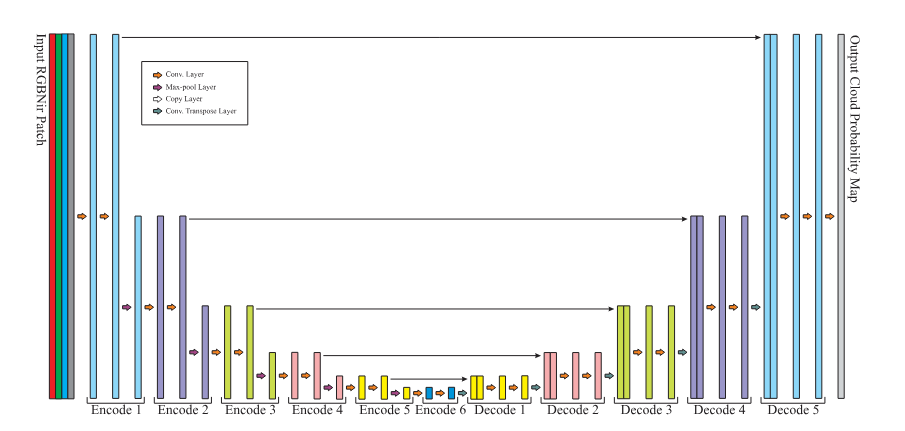
\includegraphics[width=\textwidth]{files/U-Net_cloud_detection.png}
  \caption{U-Net architecture adapted for cloud detection as used by Mohajerani et al.~\cite{mohajerani2019cloudnet}.}
  \label{fig:unet-architecture}
\end{figure}


A key innovation in U-Net is the use of residual (skip) connections \cite{he2015deepresiduallearningimage}, which dierectly link feature maps from the encoder to corresponding layers in the decoder with the same spatial size. These connections preserve fine-grained spatial details and significantly enhance segmentation quality. Moreover, they mitigate the vanishing gradient problem, facilitating the training of deeper networks and improving convergence.

\subsection{Dataset}
\label{subsec:dataset}

Landsat 8 is an Earth observation satellite launched on February 11, 2013, providing high-resolution multispectral imagery, including visible, \gls{nir}, and Thermal Infrared bands \cite{landsat8}. For cloud segmentation tasks, the \gls{rgb} and \gls{nir} channels are particularly valuable due to their ability to capture both visual and athmospheric information.

\todo{in satellite imagery add spectral ranges, explain why theyre useful for cloud detection and link datasets channels from 2.1.3 to the table of spectral ranges later, atmospheric information , clarify this. Rewrite better}

This thesis utilizes a dataset consisting of 38 annotated satellite images from the Landsat 8 mission, commonly referred to as the 38-Cloud:
A Cloud Segmentation Dataset \cite{38cloud}.
It has been introduced and adapted in the following scientific publications \cite{CloudNet2019}, \cite{CloudDet2018}.
38 images are divided into a training set containing 18 scenes and a test set with the remaining 20 scenes.
The folder structure of the dataset is illustrated below:

\begin{figure}[H]
\dirtree{%
.1 38-Cloud Dataset.
.2 38-Cloud\_training.
.3 train\_red.
.3 train\_green.
.3 train\_blue.
.3 train\_nir.
.3 train\_gt.
.3 Natural\_False\_Color.
.3 Entire\_scene\_gts.
.3 training\_patches\_38-Cloud.csv.
.3 training\_sceneids\_38-Cloud.csv.
.2 38-Cloud\_test.
.3 test\_red.
.3 test\_green.
.3 test\_blue.
.3 test\_nir.
.3 Natural\_False\_Color.
.3 Entire\_scene\_gts.
.3 test\_patches\_38-Cloud.csv.
.3 test\_sceneids\_38-Cloud.csv.
.2 training\_patches\_38-cloud\_nonempty.csv.
}
\caption{Folder structure of the 38-Cloud Dataset}
\label{fig:dsFolderStruct}
\end{figure}

Each image consists of four spectral channels: \gls{rgb} and \gls{nir}, along with a manually annotated \gls{gt} mask that labels cloud regions at the pixel level.
The four spectral channels are encoded using \glspl{uint16} per pixel, whereas the \gls{gt} masks are represented with \glspl{uint8}.
A single raw image at full resolution of approximately \ensuremath{8000\times8000} pixels would result in a file size of around 1GB.
Moreover, processing such images would require model input tensors of shape \ensuremath{batchsize\times8000\times8000\times4} in \gls{float32} after normalization.
Since efficient training typically necessitates a \ensuremath{batchsize} greater than one,
this setup would impose substantial computational demands due to increased model size and would significantly slow down both training and inference ---
making it particularly unsuitable for deployment on embedded systems.
To address this, the dataset is provided in a pre-cropped format, with each image and its corresponding \gls{gt} mask divided into 384x384 pixel patches.
These patches are saved as \code{.TIF} files within their respective channel-specific directories, such as \code{train\_red}, \code{train\_green}, and so forth.
The \gls{gt} patches for training are stored in the \code{train\_gt} directory.

\todo{maybe describe it better, to distinguish between gt train and test}

It is important to note, however, that pre-cropped \gls{gt} patches are not available for the test subset.
Instead, complete scene \gls{gt} masks are provided in the \code{Entire\_scene\_gts} directories for both the train and test subsets.

The examples of training patches from all four spectral channels and the corresponding \gls{gt} mask at a fixed location are shown below as normalized greyscale images: 

\begin{figure}[H]
  \centering
  \begin{subfigure}[t]{0.22\textwidth}
    \includegraphics[width=\linewidth]{files/examples/red_patch.png}
    \caption{Red}
  \end{subfigure}
  \hfill
  \begin{subfigure}[t]{0.22\textwidth}
    \includegraphics[width=\linewidth]{files/examples/green_patch.png}
    \caption{Green}
  \end{subfigure}
  \hfill
  \begin{subfigure}[t]{0.22\textwidth}
    \includegraphics[width=\linewidth]{files/examples/blue_patch.png}
    \caption{Blue}
  \end{subfigure}
  \hfill
  \begin{subfigure}[t]{0.22\textwidth}
    \includegraphics[width=\linewidth]{files/examples/nir_patch.png}
    \caption{NIR}
  \end{subfigure}

  \vspace{0.5em}

  \begin{subfigure}[t]{0.22\textwidth}
    \includegraphics[width=\linewidth]{files/examples/gt_patch.png}
    \caption{Ground Truth}
  \end{subfigure}

  \caption{Four spectral input patches and the corresponding ground truth mask.}
  \label{fig:patch_example}
\end{figure}

Each \gls{rgb}, \gls{nir}, and \gls{gt} patch follows a unified filename convention:

\begin{lstlisting}
<band>_patch_<index>_<row>_by_<col>_<metadata>.TIF
\end{lstlisting}

The corresponding components are:

\begin{tabularx}{0.97\textwidth}{@{\hspace{\parindent}}>{\ttfamily}p{2.7cm}@{\hspace{0.3em}}L}
\textbf{band} \dotfill & Indicates the spectral band or \gls{gt} mask. \\
\textbf{index} \dotfill & Ordinal number of the patch within the scene. Patches are extracted sequentionally from left to right, top to bottom. \\
\textbf{row \& col} \dotfill & Patch's position in the scene, specified by its row and column indices. \\
\textbf{metadata} \dotfill & Encodes the satellite and sensor ID, preprocessing precision, scene path/row, acquisition and processing dates, and collection tier metadata. \\
\end{tabularx}

An example filename:

\begin{lstlisting}
blue_patch_103_5_by_11_LC08_L1TP_063013_20160920_20170221_01_T1.TIF
\end{lstlisting}

This naming scheme ensures consistency and supports automated patch retrieval across channels.
The filenames, excluding the \code{band} prefix, are listed in the \code{training\_patches\_38-Cloud.csv} and \code{test\_patches\_38-Cloud.csv} files, respectively.
The corresponding scene-level filenames are stored in \code{training\_sceneids\_38-Cloud.csv} and \code{test\_sceneids\_38-Cloud.csv}.

One notable detail is that, due to the cropping and padding of border patches (to standardise the patch size to \ensuremath{384\times384}) and the tilted geometry of Landsat 8 imagery,
some resulting patches contain no meaningful information --- appearing completelly black with all-zero pixel values across all four channels.
These zero-information patches were excluded from the training and validation sets to avoid overrepresenting non-informative inputs,
which could degrade the model's ability to learn meaningful patterns.
The remaining useful patch names are stored in \code{training\_patches\_38-cloud\_nonempty.csv} file.

Together, these \code{.csv} files serve as the basis for dataset construction, as discussed in \secshortref{sec:data}.
Furthermore, the embedded attributes such as \code{index}, \code{row \& col} will be directly utilized during the stitching process described in \secshortref{subsec:testing}.

For visualization purposes, the full scene images are rendered using a standard false-color composite in which the \gls{nir} band is mapped to red, red band to green, and green band to blue.
This mapping coresponds to the commonly used \gls{cir} visualization in remote sensing \cite{cir1}.
\todo{check patches and scenes to verify what bands were replaced}
\gls{cir} imagery enhances features such as vegetation and clouds, which exhibit distinct reflectance patterns across the visible and \gls{nir} spectrum.
However, these false-color visualizations were not used as input for the \gls{cnn} during training, validation, or inference.
They served solely as visual references for qualitative inspection by the human observer.
The corresponding images are located in the \code{Natural\_False\_Color} directories.
An example scene is shown below as a false-color composite: 

\begin{figure}[H]
  \centering
  \includegraphics[width=0.7\textwidth]{files/examples/scene.jpg}
  \caption{False-color composite of an entire scene.}
  \label{fig:false_color_scene}
\end{figure}

\subsection{Evaluation Metrics}
\label{subsec:evalmetrics}

\subsection{Quantization}
\label{subsec:quantization}

Quantization is a mathematical method that maps a large set of (typically continuous) values to a smaller, discrete and countable set.
Its first practical application can be traced back to 1957, in the context of pulse-code modulation within the field of signal processing.
The earliest formal scientific documentation of the method appears in a publication from 1982,
which is based on a draft manuscript originally authored in 1957 \cite{firstQuantization}.

This technique is now widely employed in machine learning \cite{MLQuantization1, MLQuantization2}.
Quantization significantly reduces model size by compressing numerical precision, typically at the cost of a controlled reduction in accuracy.
\todo{add paper or image by how much model size can be reduced}
Two primary quantization methods are commonly used: general asymmetric zero-point quantization, and its special case ---
symmetric absolute maximum (absmax) quantization.
In the context of this work, the general asymetric approach is of primary importance.

To perform quantization, the boundaries \( x_{\text{min}} \) and \( x_{\text{max}} \) of the original (floating-point) range,
and \( q_{\text{min}} \) and \( q_{\text{max}} \) of the target (quantized) value set must be defined.
Once these are known, the corresponding scale and zero-point parameters are computed according to the following equations:

\begin{equation}
\text{scale} = \frac{x_{\text{max}} - x_{\text{min}}}{q_{\text{max}} - q_{\text{min}}}
\label{eq:scale}
\end{equation}

\begin{equation}
\text{zero-point} = \text{round}\left( q_{\text{min}} - \frac{x_{\text{min}}}{\text{scale}} \right)
\label{eq:zeropoint}
\end{equation}

With these parameters determined,
input value \( x \) can be transformed into quantized form \( q_{\text{x}} \) and subsequently dequantized to an approximate value \( x_{\text{q}} \) using the following formulas:

\begin{equation}
q_{\text{x}} = \text{round}\left(\frac{x}{\text{scale}} \right) + \text{zero-point}
\label{eq:quantize}
\end{equation}

\begin{equation}
x_{\text{q}} \approx \left( q_{\text{x}} - \text{zero-point} \right) \cdot \text{scale}
\label{eq:dequantize}
\end{equation}

It is essential to note that both the scale and zero-point must be preserved in order to carry out the quantization and dequantization processes.
For every value range subject to quantization, a unique pair of these parameters exists.

The following example demonstrates the use of zero-point quantization. Consider a set of continuous values ranging from -9.75 to 3.00.
To map this range onto a discrete set defined by the integer interval [-128, 127], the scale and zero-point are calculated using equations \ref{eq:scale} and \ref{eq:zeropoint}:

\begin{equation*}
\text{scale} = \frac{3.00 - (-9.75)}{127 - (-128)} = 0.05
\end{equation*}

\begin{equation*}
\text{zero-point} = \text{round}\left( -128 - \frac{-9.75}{\text{scale}} \right) = 67
\end{equation*}


After this step, every value from the original dataset can be represented by its corresponding quantized counterpart.
The following equations illustrate the quantization and subsequent dequantization of four examples using \ref{eq:quantize} and \ref{eq:dequantize}:
\( x = 0 \), \( x = 3.00 \), \( x = 2.98 \), \( x = 2.95 \):

\begin{align*}
q_{0} &= \text{round}\left(\frac{0}{0.05} \right) + 67 = 67
& \quad
x_{67} &\approx \left( 67 - 67 \right) \cdot 0.05 = 0
\end{align*}

\begin{align*}
q_{3.00} &= \text{round}\left(\frac{3.00}{0.05} \right) + 67 = 127
& \quad
x_{127} &\approx \left( 127 - 67 \right) \cdot 0.05 = 3.00
\end{align*}

\begin{align*}
q_{2.98} &= \text{round}\left(\frac{2.98}{0.05} \right) + 67 = 127
& \quad
x_{127} &\approx \left( 127 - 67 \right) \cdot 0.05 = 3.00
\end{align*}

\begin{align*}
q_{2.95} &= \text{round}\left(\frac{2.95}{0.05} \right) + 67 = 126
& \quad
x_{126} &\approx \left( 126 - 67 \right) \cdot 0.05 = 2.95
\end{align*}

The last three examples implicitly demonstrate the loss of precision introduced by quantization.
In this particular case, any input value between 2.95 and 3.00 will be represented, after conversion, by one of these two discrete values.

It is important to emphasize that the scale parameter etirely defines the quantizer's precision,
under the assumption that the bit-width (i.e., 255 discrete representable values) is fixed,
as well as the floating-point range from -9.75 to 3.00 being evenly distributed across the entire interval and free of outliers.

In practice, more advanced quantization techniques may be employed, such as outlier-aware clipping, per-axis and per-tensor quantization,
symmetric and asymmetric schemes, or methods like dynamic range adjustment and mixed-precision quantization.
While the detailed explanation of these methods falls outside the scope of this thesis,
it is important to note that such techniques are already available within various \gls{tf} utilities, which will be utilized in this work.

To quantize a deep learning model, its weights, biases, and, if required, its inputs, activations, and outputs must be quantized. This is performed through \gls{ptq}.
Due to the previously described loss of precision introduced by quantization, model effectiveness metrics may degrade.
To mitigate this, the model architecture can be adapted to perform \gls{qat} prior to \gls{ptq}.
\gls{qat} does require additional computational operations, resulting in increased training time.
It should be clarified that model training can be performed using various numerical data types for model parameters; in this work, however, \gls{float32} is used.

\subsubsection{Quantization-Aware Training}
\label{subsubsec:qat}

The model architecture is modified by inserting quantization-dequantization operations at the connections between layers,
and by applying them to weights, biases, and activations.
In the forward pass, dequantization is applied immediately after quantization for each \gls{qat}-annotated \gls{float32} value.
In this way, all values remain in \gls{float32} format for training,
but quantization inaccuracies are introduced, exposing the model to quantization effects during training and allowing it to adapt its parameters accordingly.

The rounding function essential to quantization is, however, not differentiable. For this reason, the \gls{ste} is applied during the backward pass,
setting the gradient of quantization operations to 1 within the quantized range and to 0 outside it.
This allows gradients to flow through the quantization-dequantization operations \cite{qatBackwardPass}.

At the end of \gls{qat}, the model parameters are adapted to the effects of quantization and will therefore exhibit better performance after \gls{ptq} compared to a model without \gls{qat}.

\todo{Insert Netron screenshot showing scales, quantizedwrappersV2, and bias scales in the implementation/conversion section. Explain scale and bit shifts for integer arithmetic on Coral.}

\subsubsection{Post-Training Quantization}

The actual conversion of model parameters is performed during \gls{ptq}.
Regardless of whether \gls{qat} was performed, \gls{ptq} can always be applied to quantize a model.
There are three common \gls{ptq} methods, with each subsequent method quantizing more parameters until covering all \gls{float32} values in the model:

\begin{itemize}
\item \textbf{Weight-Only Quantization}: Model weights and biases are statically determined after training;
hence, their minimum and maximum values can be directly observed and used to calculate the scales and zero-points required for quantization.
Model inputs, activations, and outputs, however, remain in \gls{float32} format. This method already reduces model size and speeds up inference.
However, additional computations are needed at runtime to interface between quantized weights/biases and \gls{float32} inputs, activations, and outputs.
\item \textbf{Dynamic Range Quantization}: This method extends weight-only quantization by quantizing the most computationally intensive
operations (such as matrix multiplications and convolutions) to use integer arithmetic.
For each such operation, the input activations are temporarily converted to a quantized format for computation, and the results are subsequently converted back to \gls{float32}.
The model inputs, activations, and outputs remain in \gls{float32} format. No explicit range estimation is needed prior to conversion,
as value ranges are determined dynamically at inference time or via heuristics. This approach offers further speed improvements with minimal impact on model accuracy.
\item \textbf{Full-Integer Quantization}: In this method, all \gls{float32} values in the neural network, including inputs, activations, and outputs, are quantized.
To accurately determine the value ranges of inputs, activations, and outputs, a representative (calibration) dataset is forward-passed through the model during conversion.
The observed extrema are then used to set the quantization parameters for every tensor in the network. A key assumption is that the real inference data will have a similar value range.
This trade-off maximally reduces model size and enables highly efficient inference using integer-only arithmetic.
\end{itemize}

\subsection{Hardware}
\label{subsec:hardware}

Running machine learning inference on embedded systems is referred to as edge inference.
The Coral dev Board Mini, developed by Google, is a compact single-board computer designed for such edge AI applications.
It features quad-core MediaTek 8167s System-on-a-Chip (SoC) on the Armv8-A architecture,
along with a dedicated Edge TPU --- a hardware accelerator optimized for executing TensorFlow Lite models using 8-bit integer operations.

The Edge TPU delivers up to 4 trillion operations per second (TOPS) of performance while consuming only around 2 watts of power,
making it ideal for use in resource-constrained environments such as satellites, where energy efficiency and reliability are crucial.

To deploy a model on Edge TPU, it must meet the following requirements:
\begin{itemize}
    \item Tensor parameters quantized in \gls{int8} or \gls{uint8}
    \item Tensor sizes are constant at compile-time
    \item Model parameters (such as bias tensors) are constant at compile-time
    \item Tensors are either 1-, 2-, or 3-dimensional. If a tensor has more than 3 dimensions, then only the 3 innermost dimensions may have a size greater than 1.
    \item The model uses only the operations supported by the Edge TPU (see table 1 below). \todo{CROP the table to only relevant commands and paste it}
\end{itemize}

These requirements directly affect model architecture, training strategy, and tooling. For instance, certain operations unsopported by Edge TPU must be avoided,
and quantization aware training or post-training quantization must be considered early in the development process.

The following image from Coral documentation summarizes the model conversion and deployment workflow.

\begin{figure}[H]
  \centering
  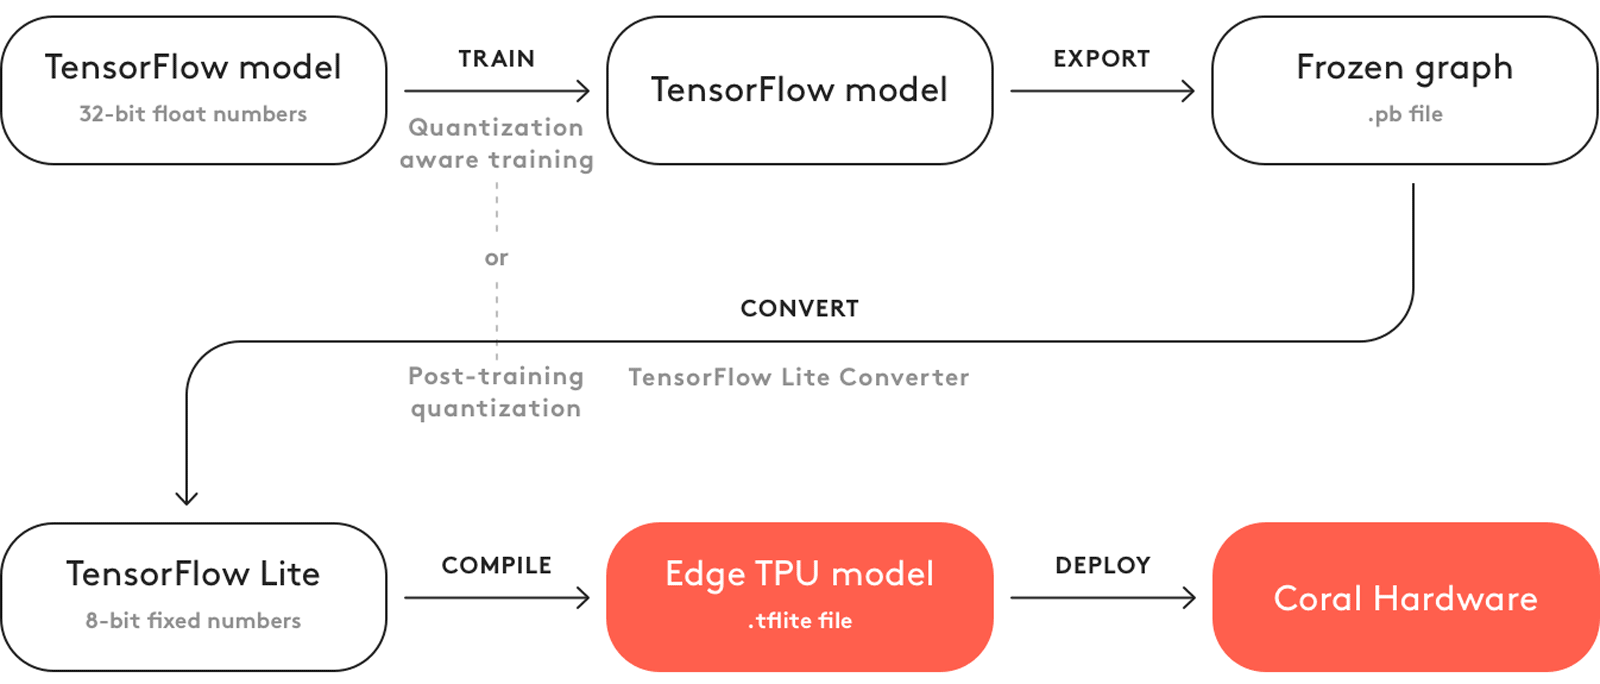
\includegraphics[width=\textwidth]{files/Edge_TPU_quantization.png}
  \caption{The basic workflow to create a model for the Edge TPU}
  \label{fig:quantization-chart}
\end{figure}

\section{Design}

\subsection*{Data}

To efficiently utilize \gls{tf}'s dataset loading and preprocessing capabilities, a versatile data handling method has to be implemented.
A core idea behind this approach is to unify the preparation of training, validation and test subsets within a single configurable function.
This function must manage all aspects of dataset construction and transformation according to user-defined parameters, thereby ensuring consistensy and flexibility.
The function should output \code{tf.data.Dataset} objects \cite{tfDataset} that are ready for immediate use in training pipelines. \cite{tfPaper}
\todo{cite main tf paper somwhere else earlier}

Ideally, the testing pipeline should also be incorporated within this flexible, unified function.
The absence of pre-cropped test subset \gls{gt} patches introduces the necessity for additional preparation steps.

\subsection*{Model}

%Separate from the dataset pipeline, the model architecture is developed independently.
The model architecture is tailored for deployment on embedded systems, where \gls{qat} must be taken into account.
Due to the lack of existing practical examples for deploying this specific model architecture on \gls{edgetpu},
the design process begins with a minimal configuration, using the smallest feasible number of layers and filters,
and gradually increases in complexity based on deployment outcomes and evaluation feedback.
An iterative, trial-and-error methodology is employed, allowing for adjustments in response to the resource constrains encountered on embedded hardware.

The objective is to implement multiple configurable functions, each responsible for constructing a distinct model architecture.
These functions include all necessary helper routines and utilities required to assemble the desired architecture,
allowing convenient switching between models during training.
%These limitations necessitate such architectural decisions, as the use of \gls{qat}.
%For this purpose, model layers are annotaded appropriately to support later quantization and efficient deployment on hardware with limited resources.

\subsection*{Training}
\label{subsec:designtrain}

After implementing utilities for dataset construction and defining the model architecture, the next step is to develop the training pipeline.
Initially, a simple and direct training pipeline should be created to validate basic model architectures, as a minimal setup both reduces potential error sources and enables rapid proof-of-concept.
During early development, model conversion is performed separately after training, before deployment.

However, the pipeline should be further refined, ideally as a single executable script, that encompasses data loading, training, configuration management, and model conversion,
streamlining the path to deployment. The goal is to enable a convenient, one-click training and conversion workflow.

To ensure reproducibility and facilitate backups, it is important to store all training configurations, logs, and intermediate model weights for each run.

Finally, computational resources must be considered. To avoid prohibitively long training times, the use of more powerful machines or cloud-based resources should be evaluated.

\subsection*{Conversion}

After training, the model must be converted and compiled for \gls{edgetpu} inference.
A modular approach is important here as well, simplifying debugging and ensuring correct conversion and compilation during early development.
Later, as described in \secshortref{subsec:designtrain}, integration of the conversion process directly into the training pipeline is ideal for convenience and efficiency.

Automation of the \gls{edgetpu} compiler,
provided by Google\footnote{\url{https://coral.ai/docs/edgetpu/compiler/}},
is required so that the entire training and conversion pipeline outputs a model ready for deployment on the \gls{devboard}.

\subsection*{Deployment}
\label{subsec:designdep}



\subsection*{Evaluation}
I wanna first conveniently have training, validation and test datasets ready for efficient TF training.
Then the convenient model architecture builder needs to be implemented
quantization aware training and post training quantization should be considered

}